In the present chapter the SPH formulations realized in GPUSPH will be
described. While this section is as complete as necessary we recommend
to read the cited literature in order to gain a full understanding of
the respective methods.

The basic premise is that GPUSPH approximates solutions to the
Navier-Stokes equations which are given by
\begin{equation}
\tdv{\uvec{v}}{t} = -\frac{1}{\rho}\nabla p + \nabla \cdot (\nu
\nabla \otimes \uvec{v}) + \uvec{g},
\label{e:sph:ns}
\end{equation}
where $\uvec{v}$ is the velocity, $\rho$ the density, $p$ the
pressure, $\nu$ the kinematic viscosity and $\uvec{g}$ an external
force. These equations are coupled with the continuity equation
\begin{equation}
\tdv{\rho}{t} = - \rho \nabla \cdot \uvec{v}.
\label{e:sph:cont}
\end{equation}
In order to close the system of equations a weakly-compressible
formulation is chosen which uses the Cole Equation of State given by
\begin{equation}
p = \frac{c_0 \rho_0}{\xi}\left[ \left( \frac{\rho}{\rho_0}\right)^\xi
-1 \right],
\label{e:sph:eos}
\end{equation}
where $c_0$ is the speed of sound, $\rho_0$ the reference density and
$\xi$ is the polytropic index, equal to 7 in the case of water.

\section{The SPH approximation}

At the heart of the SPH method is an interpolation that defines a
physical quantity at a certain position. Let $f$ be such a quantity,
then
\begin{equation}
f(r) = \int f(s) \delta(\|r-s\|) \td s,
\label{e:sph:delta}
\end{equation}
where $\delta$ is the Dirac delta distribution. The continuous SPH
approximation can be written as
\begin{equation}
[f]^c(r) = \int_\Omega f(s) w(\|r-s\|,h) \td s,
\label{e:sph:cint}
\end{equation}
where the Dirac delta function was replaced by a weight or kernel
function $w$, $\Omega$ is the computational domain and $h$ is the
smoothing length. Several constraints are imposed on this function
\begin{itemize}
\item $\underset{h\rightarrow 0}{\lim} w(.,h) = \delta(.)$, \ie the
kernel function converges to the delta function,
\item $\int w(s,h) \td s = 1$, \ie the kernel function has unitary
integral,
\item $w(s,h) = w(-s,h)$, \ie the kernel is symmetric,
\item the kernel has compact support.
\end{itemize}
The continuous interpolation of Eq. \eqref{e:sph:cint} does not yet
contain any discretization of space. In SPH the computational domain is
discretized using points in space that have no explicit connection with
each other. These points carry the physical information such as density
and volume and are referred to as particles. They also carry a mass and
thus have an associated volume. The position of a particle is denoted
with $\uvec{r}_a$ where the subscript $a$ refers to particle $a$.
Similarly any physical quantity is subscripted in order to refer to the
particle, \eg $\rho(\uvec{r}_a) = \rho_a$.

Now that the space has been discretized the continuous interpolation
(Eq. \eqref{e:sph:cint}) can be converted by replacing the integral with
a sum to yield the SPH interpolation as
\begin{equation}
[f]_a = \underset{b \in \mathcal{F}}{\sum} \frac{m_b}{\rho_b} f_b w_{ab},
\label{e:sph:int}
\end{equation}
where $\mathcal{F}$ is the set of all particles, $m$ the mass and
$w_{ab} = w(\|\uvec{r}_a - \uvec{r}_b\|/h, h)$. It should be noted that
$[f]_a \neq f_a$, \ie SPH violates the Kronecker delta property.

\subsection{SPH kernels}

Currently GPUSPH features four different kernels.
\begin{itemize}
  \item \cmd{CUBICSPLINE}: The cubic spline function
  \item \cmd{QUADRATIC}:
  \item \cmd{WENDLAND}: The quintic Wendland function
  \item \cmd{GAUSSIAN}: The Gaussian
\end{itemize}

The formulae for the different kernels and their derivatives are given below.

The Wendland kernel is given by
\begin{equation}
w(q,h) = \left\{ \begin{array}{rl}
 \dfrac{\alpha_W}{h^3} \left(1-\dfrac{q}{2}\right)^4(1+2q) &\mbox{ if $0\le q \le 2$,} \\
  0 &\mbox{ if $2 < q$,}
       \end{array} \right.
\label{e:sph:wendland}
\end{equation}
where $\alpha_W = 21/(16\pi)$ and its derivative by
\begin{equation}
\|\nabla w(q,h)\| = \left\{ \begin{array}{rl}
  \dfrac{\alpha_{\nabla W}}{h^5}\left(q-2\right)^3 &\mbox{ if $0\le q \le 2$,} \\
  0 &\mbox{ if $2 < q$,}
       \end{array} \right.
\label{e:sph:gradwendland}
\end{equation}
where $\alpha_{\nabla W} = 105/(128\pi)$ in 3-D.

\todo{Complete kernel information}

\subsection{First-order derivatives}

In order to approximate derivatives the continuous SPH interpolation Eq.
\eqref{e:sph:cint} is used as follows
\begin{equation}
[\nabla f]^c(r) = \int_\Omega \nabla f(s) w(\|r-s\|,h) \td s.
\label{e:sph:cint-gradf-start}
\end{equation}
Applying integration by parts yields
\begin{equation}
[\nabla f]^c(r) = - \int_\Omega f(s) \nabla_s w(\|r-s\|,h) \td s +
\int_\Omega \nabla (f(s) w(\|r-s\|,h)) \td s.
\label{e:sph:cint-intpart}
\end{equation}
As $w$ is symmetric the kernel is antisymmetric and thus
\begin{equation}
\nabla_s w(\|r-s\|,h) = - \nabla_r w(\|r-s\|,h).
\label{e:sph:kernel-asym} \end{equation}
Furthermore, using Stokes
theorem the last term in Eq. \eqref{e:sph:cint-intpart} can be rewritten
as integral over the boundary of the computational domain, denoted by
$\partial \Omega$ which yields
\begin{equation}
[\nabla f]^c(r) = \int_\Omega f(s) \nabla_r w(\|r-s\|,h) \td s -
\int_{\partial\Omega} (f(s) w(\|r-s\|,h)) \uvec{n}_s \td s,
\label{e:sph:cint-stokes}
\end{equation}
where $\uvec{n}_s$ is the inward pointing normal. As a convention for
the remainder of this document all normals will point inward the domain.
If the domain $\Omega$ is unbounded then the last term of Eq.
\eqref{e:sph:cint-stokes} will vanish due to the compact support of the
kernel $w$. Thus, in a continuous sense the first derivative can be
approximated as
\begin{equation}
[\nabla f]^c(r) = \int_\Omega f(s) \nabla_r w(\|r-s\|,h) \td s.
\label{e:sph:cint-gradf}
\end{equation}
The discretization in space again replaces the integral by a sum over
all particles and so
\begin{equation}
[\nabla f]_a = \sumF V_b f_b \nabla_a w_{ab},
\label{e:sph:int-gradf}
\end{equation}
where $V_b = m_b/\rho_b$ is the volume of a particle $b$. It is common
in SPH practice to write the gradient operator slightly different as it
is used to compute the pressure gradient and thus Newtons third law of
equal but opposite forces should be obeyed. This can be achieved by
defining the gradient as
\begin{equation}
\Grad_a(f) = [\nabla f]_a + [\nabla f_a]_a,
\label{e:sph:grad-def}
\end{equation}
where the latter derivative is that of a constant function $f_a$. As
derivatives of constant functions are not necessarily zero this term
will have a non-zero contribution.

\todo{Add different formulations SPH_F1 and SPH_F2, including theory}

The principle of energy conservation requires the gradient and
divergence operators to be skew-adjoint, \ie
\begin{equation}
<\Grad_a(f), \uvec{G}> = - <f, \Div_a(\uvec{G})>,
\label{e:sph:skew-ajd}
\end{equation}
where $<.,.>$ is a scalar product on all particles. As a result of this
constraint the divergence can be shown to be
\begin{equation}
\Div_a(\uvec{G}) = [\nabla \uvec{G}]_a - [\nabla \uvec{G}_a]_a.
\label{e:sph:div-def}
\end{equation}
This allows to write the gradient and divergence as
\begin{equation}
\Grad_a(f) = \sumF V_b (f_b + f_a) \nabla_a w_{ab},
\label{e:sph:grad}
\end{equation}
and
\begin{equation}
\Div_a(\uvec{G}) = \sumF V_b (\uvec{G}_b - \uvec{G}_a) \cdot \nabla_a w_{ab},
\label{e:sph:div}
\end{equation}
respectively.

\subsection{Second-order derivatives}

In theory second-order derivatives could simply be derived from first
order ones, but that would cause second derivatives to appear which are
numerically unstable. Thus, the preferred approach is to use a
combination of a SPH first order derivative and a finite difference
first order derivative.

The goal of this section is to derive a discretization for $\nabla f
\nabla \otimes \uvec{G}$. To approximate the interior gradient, a
Taylor Series of $\uvec{G}$ can be used as follows
\begin{equation}
\uvec{G}_b = \uvec{G}_a - (\nabla_a \otimes \uvec{G})^T \cdot
\uvec{r}_{ab} + \mathcal{O}(\uvec{r}_{ab}),
\label{e:sph:taylor}
\end{equation}
where $\uvec{r}_{ab} = \uvec{r}_a - \uvec{r}_b$, a convention that will
be used throughout this document also for quantities different from
$\uvec{r}$.
The above can be rewritten to obtain an expression for the interior
gradient
\begin{equation}
(\nabla_a \otimes \uvec{G})^T \cdot
\frac{\uvec{r}_{ab}}{\|\uvec{r}_{ab}\|} \approx
\frac{1}{\|r_{ab}\|}\uvec{G}_{ab},
\label{e:sph:grad-finitediff}
\end{equation}
and similarly
\begin{equation}
(\nabla_b \otimes \uvec{G})^T \cdot
\frac{\uvec{r}_{ab}}{\|\uvec{r}_{ab}\|} \approx
\frac{1}{\|r_{ab}\|}\uvec{G}_{ab},
\label{e:sph:grad-finitediff-b}
\end{equation}
As the kernel is radially symmetric
\begin{equation}
\nabla_a w_{ab} = \frac{\uvec{r}_{ab}}{\|\uvec{r}_{ab}\|} \|\nabla_a
w_{ab}\|.
\label{e:sph:rad-sym}
\end{equation}
The Divergence similar to the one given by Eq.
\eqref{e:sph:div} but with a $+$ instead of the $-$ yields
\begin{equation}
\nabla \cdot (f \nabla \otimes \uvec{G}) = \sumF V_b (f_b \nabla_b
\otimes \uvec{G} + f_a \nabla_a \otimes \uvec{G})
\frac{\uvec{r}_{ab}}{\|\uvec{r}_{ab}\|} \|\nabla_a w_{ab}\|,
\end{equation}
which, with Eqs. \eqref{e:sph:grad-finitediff},
\eqref{e:sph:grad-finitediff-b} and \eqref{e:sph:rad-sym}, can be used to
define the Laplacian
\begin{equation}
\Lap_a(f, \uvec{G}) = \nabla \cdot (f \nabla \otimes \uvec{G}) = \sumF
V_b (f_b + f_a) \uvec{G}_{ab} \frac{1}{\|\uvec{r}_{ab}\|} \|\nabla_a w_{ab}\|.
\label{e:sph:lap}
\end{equation}

\subsection{Discretization of the Navier-Stokes equations}
With the definition of the three operators $\Grad$, $\Div$ and $\Lap$ as
given by Eqs. \eqref{e:sph:grad}, \eqref{e:sph:div} and
\eqref{e:sph:lap}, respectively, the Navier-Stokes equations
\eqref{e:sph:ns} and \eqref{e:sph:cont} can be discretized in space as
\begin{eqnarray}
\tdv{\uvec{v}_a}{t} &=& - \frac{1}{\rho_a}\Grad_a(p) +
\Lap_a(\nu,\uvec{v}) + \uvec{g},
\label{e:sph:ns-disc}
\\
\tdv{\rho_a}{t} &=& -\rho_a \Div_a(\uvec{v}).
\label{e:sph:cont-disc}
\end{eqnarray}
The final step to a full discretization is the implementation of a time
integration scheme. GPUSPH currently features a predictor-corrector
scheme that is given by
\begin{eqnarray}
\uvec{u}^{n+1/2} &=& \uvec{u}^n + \frac{\Delta t}{2} NS(\uvec{u}^n),
\label{e:sph:pred-corr}
\\
\uvec{u}^{n} &=& \uvec{u}^n + \Delta t NS(\uvec{u}^{n+1/2}),
\nonumber
\end{eqnarray}
where $\uvec{u}$ is the state vector and $NS$ are the right-hand sides
of the discretized Navier-Stokes equations. Furthermore, the
superscripts refer to the time instances. Written out in detail
the full discretization reads
\begin{eqnarray}
\uvec{v}_a^{n+1/2} &=& \uvec{v}_a^n + \frac{\Delta t}{2} \left(
-\frac{1}{\rho^n_a}\Grad_a(p^n) + \Lap_a(\nu^n,\uvec{v}^n) + \uvec{g}
\right),
\label{e:sph:pred-corr-ns}
\\
\uvec{r}_a^{n+1/2} &=& \uvec{r}_a^{n} + \frac{\Delta t}{2}
\uvec{v}_a^{n},
\nonumber
\\
\rho_a^{n+1/2} &=& \rho_a^n - \frac{\Delta t}{2} \rho_a^n
\Div_a(\uvec{v}^n),
\nonumber
\\
p_a^{n+1/2} &=& \frac{c_0 \rho_0}{\xi}\left[ \left( \frac{\rho_a^{n+1/2}}{\rho_0}\right)^\xi
-1 \right],
\nonumber
\\
\uvec{v}_a^{n+1} &=& \uvec{v}_a^n + \Delta t \left(
-\frac{1}{\rho^{n+1/2}_a}\Grad_a(p^{n+1/2}) +
\Lap_a(\nu^{n+1/2},\uvec{v}^{n+1/2}) + \uvec{g}
\right),
\nonumber
\\
\uvec{r}_a^{n+1} &=& \uvec{r}_a^{n} + \Delta t\,
\uvec{v}_a^{n+1/2},
\nonumber
\\
\rho_a^{n+1} &=& \rho_a^n - \Delta t\, \rho_a^{n+1/2}
\Div_a(\uvec{v}^{n+1/2}),
\nonumber
\\
p_a^{n+1} &=& \frac{c_0 \rho_0}{\xi}\left[ \left( \frac{\rho_a^{n+1}}{\rho_0}\right)^\xi
-1 \right].
\nonumber
\end{eqnarray}

\subsubsection{Alternative continuity equation}
The density can alternatively be computed by
\begin{equation}
[\rho]_a = \sumF V_b \rho_b w_{ab},
\end{equation}
which simplifies to
\begin{equation}
[\rho]_a = \sumF m_b w_{ab}.
\label{e:sph:sumrho}
\end{equation}
To be consisten with the time-stepping and to preserve initial density
values the following time dependent version is used
\begin{equation}
\rho_a^{n+1} = \rho_a^n - \left(\sumF m_b w_{ab}\right)^n + \left(\sumF
m_b w_{ab}\right)^{n+1},
\label{e:sph:sumrho-time}
\end{equation}
where the sums inside the brackets are with respect to the positions of
the particles at the respective time step indicated by the superscript.
It can be shown \todo{cite vila} that this is equivalent to the
continuity equation based on the divergence. However, as the formulation
depends only on the particle position it is numerically more stable.

\section{Boundary conditions}\label{sec:boundary_conditions}

Several different boundary conditions are available for the SPH method
and a few selected ones are implemented in GPUSPH. Currently the
following options are implemented
\begin{itemize}
  \item \cmd{LJ_BOUNDARY}: Lennard-Jones boundary conditions
  \item \cmd{MK_BOUNDARY}: Monaghan-Kajtar boundary conditions
  \item \cmd{SA_BOUNDARY}: Semi-analytical boundary conditions
  \item \cmd{DYN_BOUNDARY}: Dynamic boundary conditions
\end{itemize}
In the following these boundary conditions and their formulations will
be described in detail.

\subsection{Semi-analytical boundaries}

The semi-analytical wall boundary conditions developed by Ferrand \etal
\cite{ferrand_unified_2012} have shown promising results in the
simulation of flows with complex boundaries using the Smoothed Particle
Hydrodynamics (SPH) method. Recent efforts have pushed these boundary
towards practical applications \cite{mayrhofer_unified_2014, leroy_unified_2014}.
While the accuracy of these boundary conditions is outstanding, one of
their downsides is their comparably high computational cost.
\begin{figure}[htb]
\centering
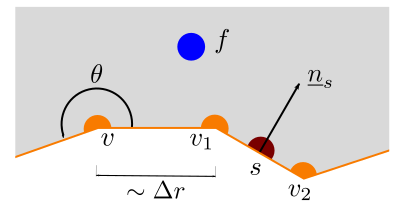
\includegraphics[width=0.48\textwidth]{fig/vertex_and_boundary_elements.pdf}
\caption{Different particle types}
\label{fig:sa:types}
\end{figure}
The domain $\Omega$ which is the fluid domain is discretized using three different sets of particles:
\begin{enumerate}
\item $f \in \mathcal{F}$: the fluid particles,
\item $p \in \mathcal{P}$: the vertex particles,
\item $s \in \mathcal{S}$: the boundary elements.
\end{enumerate}
The boundary segments are triangles, in the 3-D case, that are located at the boundary $\partial \Omega$ of the domain. At each vertex of such a boundary elements is a vertex particle that has a mass that is related to the boundary shape as shown in Fig. \ref{fig:sa:types}. These particles, in a finite volume sense, represent the near-wall cells and are moving only if the solid wall is. The fluid particles on the other hand are typical SPH particles that move in a Lagrangian fashion and occupy $\Omega$. The union of fluid and vertex particles will be denoted with $\mathcal{P}$.

The SPH interpolation in the context of the semi-analytical boundary conditions is given by
\begin{equation}
[f]_a = \frac{1}{\gamma_a}\sumP V_b f_b w_{ab},
\label{e:sa:int}
\end{equation}
where $\gamma_a$ is the kernel renormalization parameter defined as
\begin{equation}
\gamma_a = \int_\Omega w(\|\uvec{r}-\uvec{r_b}\|),
\label{e:sa:gam}
\end{equation}
which is computed following the idea by Violeau \etal
\cite{violeau_exact_2014}. However, instead of analytically evaluating
the integral over the boundary element, a \nth{5}-order quadrature rule
is used. Note that currently this is implemented only for the Wendland
kernel and so the semi-analytical boundary conditions can only be used
using this kernel.

The differential operators gradient and divergence are given as
\begin{eqnarray}
\Grad_a(p) &=& \frac{1}{\gamma_a}\sumP V_b (p_a+p_b) \nabla_a w_{ab}
 -\frac{1}{\gamma_a}\sumS (p_a + p_s) \nabla \gamma_{as},
\label{e:sa:grad}
\\
\Div_a(\uvec{v}) &=& \frac{1}{\gamma_a}\sumP V_b (\uvec{v}_b - \uvec{v}_a) \cdot \nabla_a w_{ab}
 -\frac{1}{\gamma_a}\sumS (\uvec{v}_s - \uvec{v}_a) \cdot \nabla \gamma_{as},
\label{e:sa:div}
\end{eqnarray}
respectively. $\nabla \gamma_{as}$ is the surface integral of the kernel
on a triangle $s$ which is solved using the same \nth{5}-order
quadrature rule. The derivation of these operators can be found in
\cite{ferrand_unified_2012}. The basic idea is to not drop the surface
integral term in Eq. \eqref{e:sph:cint-stokes} but instead replace it
with a discrete approximation, \ie the sum over the segments. The Laplacian operator, required to discretize the viscous term of the momentum equation, is given by
\begin{equation}
\Lap_a(\nu, \uvec{v}) = \frac{1}{\gamma_a}\sumP m_b \left(\frac{\nu_a}{\rho_b} + \frac{\nu_b}{\rho_a}\right) \frac{\uvec{v}_{ab}}{\|\uvec{r}_{ab}\|^2}\uvec{r}_{ab}\cdot \nabla_a w_{ab}
 - \frac{2 \nu_a \uvec{v}_a}{\gamma_a} \sumS \frac{\|\nabla \gamma_{as}\|}{\delta r_{as}},
\label{e:sa:lap}
\end{equation}
where the laminar shear stress was used in the boundary term \cite{ferrand_unified_2012}, $\uvec{r}_{ab} = \uvec{r}_a - \uvec{r}_b$ and $\delta r_{as} = \max(\uvec{r}_{as}\cdot\uvec{n}_s, \Delta r)$. Finally the Dirichlet boundary condition $\uvec{v} = 0$ is applied at no-slip boundaries by imposing $\uvec{v}_a = 0\ \forall a \in \mathcal{V} \cup \mathcal{S}$. The Neumann boundary condition $\partial \rho/\partial \uvec{n} = 0$ is imposed using the approximation
\begin{equation}
\rho_a = \frac{1}{\alpha_a}\sumF m_b w_{ab},
\end{equation}
\todo{hydrostatic correction}
with
\begin{equation}
\alpha_a = \sumF V_b w_{ab},
\label{e:sa:alpha}
\end{equation}
for all vertex particles and boundary elements (for details see \cite{mayrhofer_investigation_2013}).

The alternative continuity equation can also be extended in order to
take boundaries into account via
\begin{equation}
\rho_a^{n+1} = \frac{1}{\gamma_a^{n+1}}\left[\gamma_a^n \rho_a^n - \left(\sumF m_b
w_{ab}\right)^n + \left(\sumF\right]
m_b w_{ab}\right)^{n+1}.
\label{e:sa:sumrho-time}
\end{equation}

\todo{Add other boundary conditions}

\section{Stabilizing methods}

Due to the collocated nature of the SPH method it is unavoidable that
spurious pressure modes are created. In order to prevent the numerical
solution from becoming unstable several stabilizing methods can be
employed.

\subsection{Ferrari}

The Ferrari correction is based on the work by \todo{cite ferrari}
and modifies the continuity equation with an additional term given by
\begin{equation}
\tdv{\rho_a}{t} = -\rho_a \Div_a(\uvec{v}) + \eta_F \sumF V_b c_{a,b}\frac{\uvec{r}_{ab}}{r_{ab}}\rho_{ab}\cdot\nabla_a w_{ab},
\label{e:ferrari:cont}
\end{equation}
where
\begin{equation}
c_{a,b} = \max(c_a,c_b),
\label{e:ferrari:upw}
\end{equation}
and
\begin{equation}
c_a = c_0\sqrt{\left(\frac{\rho_a}{\rho_0}\right)^{\xi-1}}.
\label{e:ferrari:ca}
\end{equation}
Note that in the case of the semi-analytical boundaries the formulation
is the same and not boundary term needs to be added.

In certain flows (\eg direct numerical simulation of turbulent flow
\todo{cite my turb paper}) the induced diffusivity can be too high.
A more appropriate damping can be introduced by using a damping
coefficient $\eta_F$ different from one.
\cite{mayrhofer_investigation_2013} have shown that it should be chosen
according to
\begin{equation}
\eta_F = \frac{L}{10^3 \Delta r},
\label{e:ferrari:eta}
\end{equation}
where $L$ is a typical length-scale of the flow. In GPUSPH $L$ can be
set directly using the \cmd{ferrariLengthScale} variable.

\subsection{Rhie and Chow}

Similar to the Ferrari correction is the correction in the spirit of
Rhie and Chow \todo{cite them}. Again an additional term is added to the
continuity equation. However, the density at time $n+1$ is computed
first, denoted by $\widetilde{\rho}^{n+1}$, by solving the continuity
equation and then a correction is applied to obatin $\rho^{n+1}$. This
correction is given by
\begin{equation}
\rho_a^{n+1} = \eta_{RC} \widetilde{\rho}^{n+1} \left[ \Lap_a\left(
\frac{\Delta t}{\widetilde{\rho}}, \widetilde{\rho}
\right) - \Lap_a (\Delta t, \uvec{g}\cdot\uvec{r})\right],
\label{e:rc}
\end{equation}
where $\eta_{RC}$ governs the strength of this correction, but is
usually equal to one.

\todo{Add other diffusion stuff, artificial viscosity, sheppard etc.}

\section{Turbulence modelling}

\subsection{The $k-\epsilon$ model}

The $k-\epsilon$ model is a Reynolds-Averaged Navier Stokes (RANS) model that
uses two additional differential equations to close the equations
\cite{pope_turbulent_2001}. The RANS equations modify the momentum
equations as follows:
\begin{equation}
\tdv{\uvec{v}}{t} = - \frac{1}{\rho}\nabla p + \nabla \cdot ( (\nu +
\nu_T) \nabla \otimes \uvec{v}) + \uvec{g},
\label{e:turb:ns}
\end{equation}
where $\nu_T$ is the turbulent viscosity. This in turn is given by
\begin{equation}
\nu_T = C_\mu \frac{k^2}{\epsilon},
\label{e:turb:nut}
\end{equation}
where $k$ is the turbulent kinetic energy and $\epsilon$ the turbulent
dissipation. The constants, such as $C_\mu$ are summarized in Table
\ref{tab:turb:consts}. Both $k$ and $\epsilon$ are given by two
differential equations:
\begin{equation}
\tdv{k}{t} = P - \epsilon + \nabla \cdot \left[  \left(\nu +
\frac{\nu_T}{\sigma_k}\right) \nabla k\right],
\label{e:turb:k}
\end{equation}
and
\begin{equation}
\tdv{\epsilon}{t} =\frac{\epsilon}{k}\left[ C_{\epsilon_1} P -
C_{\epsilon_2} \epsilon \right]+ \nabla \cdot \left[  \left(\nu +
\frac{\nu_T}{\sigma_\epsilon}\right) \nabla k\right],
\label{e:turb:eps}
\end{equation}
where $P$ is the production, given by
\begin{equation}
P = \min(\sqrt{C_\mu} k S, \nu_T S^2),
\label{e:turb:strain}
\end{equation}
with $S$ is the scalar mean rate-of-strain $S = \sqrt{2 \uvec{\uvec{S}}
: \uvec{\uvec{S}}}$.
\begin{table}
\centering
\begin{tabular}{| c | c | c | c | c | c |}
\hline
$C_\mu$ & $\sigma_k$ & $\sigma_\epsilon$ & $C_{\epsilon_1}$ &
$C_{\epsilon_2}$ & $\kappa$
\\
\hline
0.09 & 1.0 & 1.3 & 1.44 & 1.92 & 0.41
\\
\hline
\end{tabular}
\caption{Constants of the $k-\epsilon$ model}
\label{tab:turb:consts}
\end{table}
Finally, the boundary conditions for $k$ and $\epsilon$ at solid walls
need to be prescribed. For $k$ a von Neumann boundary condition is
imposed
\begin{equation}
\pdv{k}{n} = 0.
\label{e:turb:k-bound}
\end{equation}
$\epsilon$ close to the wall can be approximated via the theoretical
relation
\begin{equation}
\epsilon = \frac{u_k^3}{\kappa z},
\label{e:turb:eps-nearwall}
\end{equation}
where $u_k = C_\mu^{1/4} \sqrt{k}$ and $z$ is the normal distance to the
wall. Clearly, this formula is singular at the wall and $\epsilon$
varies strongly when close to the wall. The flow is rather sensitive to
this value and thus proper boundary conditions are essential. In the
following section about the implementation of the $k-\epsilon$ model
with the semi-analytical boundary model this can be taken into account.

\subsubsection{Semi-analytical boundaries}
The discretization presented in the present section is based on the work
by \cite{leroy_unified_2014} and for the exact derivation the interested
reader is referred to this paper.

To discretize the equations for $k$ and $\epsilon$ the production term
requires the computations of the strain rate, which can be achieved by
using the gradient operator. However, not the one of Eq.
\eqref{e:sa:grad} is used, but instead the zero-order accurate version
given by
\begin{equation}
\Grad^-_a(\uvec{v}) = - \frac{1}{\gamma_a}\sumP V_b \uvec{v}_{ab} \otimes \nabla_a w_{ab}
 +\frac{1}{\gamma_a}\sumS \uvec{v}_{ab} \otimes \nabla \gamma_{as},
\label{e:turb:grad-}
\end{equation}
One important change compared to the laminar simulation is that the
vertex particles now also carry a velocity which is evolved according to
the viscous term, \ie
\begin{equation}
\tdv{\uvec{v}_v}{t} = \Lap(\nu + \nu_T, \uvec{v})
\label{e:turb:vert-vel}
\end{equation}
The normal component of this velocity is set to zero to avoid particles
penetrating the wall. The laplacian of the viscous term presented in Eq.
\eqref{e:sa:lap} assumes a laminar flow profile and thus needs to be
modified for turbulent flows in order to properly take the log law into
account. This is achieved by setting the Laplacian to
\begin{equation}
\Lap_a(\nu, \uvec{v}) = \frac{1}{\gamma_a}\sumP m_b \left(\frac{\nu_a}{\rho_b} + \frac{\nu_b}{\rho_a}\right) \frac{\uvec{v}_{ab}}{\|\uvec{r}_{ab}\|^2}\uvec{r}_{ab}\cdot \nabla_a w_{ab}
 - \frac{2}{\gamma_a} \sumS u_{*,as}^2 \uvec{t}_{as} \|\nabla \gamma_{as}\|,
\label{e:turb:lap}
\end{equation}
where $u_{*,as}$ is the friction velocity at the wall seen by particle
$a$ computed iteratively from the implicit equation
\begin{equation}
\frac{\uvec{v}_{as}\cdot\uvec{t}_{as}}{u_{*,as}} =
\frac{1}{\kappa}\ln\left( \frac{\delta r_{as} u_{*,as}}{\nu} \right) +
5.2,
\label{e:turb:fric-vel}
\end{equation}
where
\begin{equation}
\uvec{t}_{as} = \frac{\uvec{v}_{as} -
(\uvec{v}_{as}\cdot\uvec{n}_s)\uvec{n}_s}{\|\uvec{v}_{as} -
(\uvec{v}_{as}\cdot\uvec{n}_s)\uvec{n}_s\|}.
\label{e:turb:tas}
\end{equation}
The other term in the governing equations for $k$ and $\epsilon$ is the
Laplacian which are discretized as follows:
\begin{equation}
\Lap_a(\nu + \frac{\nu_T}{\sigma_k}, k) = \frac{1}{\gamma_a}\sumP V_b
\left( 2\nu + \frac{\nu_{T,a} + \nu_{T,b}}{\sigma_k} \right)
\frac{k_{ab}}{r_{ab}^2}\uvec{r}_{ab}\cdot \nabla_a w_{ab},
\label{e:turb:k-lap-sa}
\end{equation}
and
\begin{equation}
\Lap_a(\nu + \frac{\nu_T}{\sigma_\epsilon}, \epsilon) = \frac{1}{\gamma_a}\sumP V_b
\left( 2\nu + \frac{\nu_{T,a} + \nu_{T,b}}{\sigma_\epsilon} \right)
\frac{\epsilon_{ab}}{r_{ab}^2}\uvec{r}_{ab}\cdot \nabla_a w_{ab} +
\frac{4 C_\mu}{\sigma_\epsilon \gamma_a}\sumS\frac{k_a^2}{\delta
r_{as}}\|\nabla \gamma_{as}\|.
\label{e:turb:eps-lap-sa}
\end{equation}
The compatible values on the boundary are given by
\begin{equation}
k_v = \frac{1}{\alpha_v}\sumF V_b k_b w_{vb},
\label{e:turb:k-bound-sa}
\end{equation}
and
\begin{equation}
\epsilon_v = \frac{1}{\alpha_v}\sumF V_b \left( \epsilon_b +
\frac{4 C_\mu^{3/4} k_b^{3/2}}{\kappa \delta r_{bv}} \right) w_{vb},
\label{e:turb:eps-bound-sa}
\end{equation}
where $\alpha_v$ is given according to Eq. \eqref{e:sa:alpha}.

\todo{Add SPS}

\section{Open boundaries}
GPUSPH currently implements two different types of open boundaries. One
of them is for the dynamic boundary conditions and uses a buffer zone
approach. The other can only be used in conjunction with the
semi-analytical boundary conditions and uses flat open boundaries, which
allows for in- and outflow to be at the same wall (\eg waves).

\subsection{Semi-analytical open boundaries}

The open boundaries are based around the idea of vertex particles with
varying mass. The mass of these vertex particles can change due to three
different reasons:
\begin{itemize}
\item Flux through the boundary
\item Fluid particle crossing boundary
\item Creation of new fluid particle
\end{itemize}
An open boundary has either a prescribed velocity or a prescribed
pressure and in the following these two options will be denoted with
velocity and pressure boundary, respectively. The quantity that is not
prescribed needs to be computed using Riemann invariants which is
detailed in the following.

\subsubsection{Riemann invariants for velocity boundaries}
\label{h:open:vel}
The imposed normal velocity at the open boundary is denoted with
$u_{ext}$. The normal velocity inside the flow is extrapolated to the wall
by
\begin{equation}
u_{int,a} = \frac{1}{\alpha_a}\sumF V_b \uvec{v}_b \cdot \uvec{n}_a
w_{ab}.
\label{e:open:uint}
\end{equation}
Similary, the pressure is extrapolated according to
\begin{equation}
p_{int,a} = \frac{1}{\alpha_a}\sumF V_b p_b w_{ab}.
\label{e:open:pint}
\end{equation}
$\rho_{int}$ can easily be computed using the inverse Equation of State
($EOS^{-1}$). The aim of this section will be to compute $p_{ext,a}$
from the extrapolated and imposed quantities.

The main idea is that there is an internal and an external state with
the interface at the open boundary. Due to the discontinuity of the
internal and external fields and the assumption of a 1-D problem the
Riemann problem is recovered and a solution is known that can be divided
into three different states.

Let
\begin{equation}
\psi(\rho) = \frac{2 c_0}{\xi - 1}\left( \frac{\rho}{\rho_0}
\right)^{\frac{\xi-1}{2}}\mbox{ if } \xi > 1 \quad \mbox{ or } \quad
\psi(\rho) = c_0 \ln\left( \frac{\rho}{\rho_0} \right) \mbox{ if } \xi =
1.
\label{e:open:psi}
\end{equation}
and $\psi^{-1}$ the respective inverse function. The three states yield
the following densities
\begin{itemize}
  \item Expansion wave:
  \begin{equation}
  \rho_{ext,e} = \psi^{-1}(\psi(\rho_{int}) +
  u_{ext} - u_{int})
  \label{e:open:vexp}
  \end{equation}
  \item Shock wave:
  \begin{equation}
  \rho_{ext,s} = EOS^{-1}(p_{int} + \rho_{int}
  u_{int} (u_{int} - u_{ext}))
  \label{e:open:vshock}
  \end{equation}
  \item Contact discontinuity
  \begin{equation}
  \rho_{ext,c} = \rho_{int}
  \label{e:open:vcontact}
  \end{equation}
\end{itemize}
To decide which state needs to be considered the speed of sound as
function of density needs to be defined as
\begin{equation}
c(\rho) = c_0 \left( \frac{\rho}{\rho_0} \right)^{\frac{\xi - 1}{2}}
\label{e:open:speedofsound}
\end{equation}
to be able to compute the celerities $\lambda$. They are given as
\begin{eqnarray}
\lambda &=& u_{int} + c(\rho_{int}),
\label{e:open:lambda}
\\
\lambda_e &=& u_{ext} + c(\rho_{ext,e}),
\label{e:open:vlambda_e}
\\
\lambda_s &=& u_{ext} + c(\rho_{ext,s}),
\label{e:open:vlambda_s}
\end{eqnarray}
Based on these celerities the states occur according to
\begin{itemize}
  \item $\lambda_e \le \lambda \Rightarrow$ expansion wave
  \item $\lambda_s > \lambda \Rightarrow$ shock wave
  \item $\lambda_e > \lambda \ge \lambda_s \Rightarrow$ contact
  discontinuity
\end{itemize}
Depending on the computed state the pressure $p_{ext}$ is set according
to the corresponding density in Eqs. \eqref{e:open:vexp},
\eqref{e:open:vshock} or \eqref{e:open:vcontact}.

\subsubsection{Riemann invariants for pressure boundaries}
\label{h:open:pres}
Compared to the velocity boundary, this time $u_{ext}$ needs to be
computed and $p_{ext}$ is imposed. Similar to the previous section three
different fluxes, $u_{ext}$, can be computed according to the different
states
\begin{itemize}
\item Expansion wave:
\begin{equation}
u_{ext,e} = u_{int} + \psi(\rho_{ext}) - \psi(\rho_{int})
\label{e:open:pexp}
\end{equation}
\item Shock wave:
\begin{equation}
u_{ext,s} = u_{int} + \frac{p_{int} - p_{ext}}{\rho_{int}\max(u_{int},
10^{-5}c_0)}
\label{e:open:pshock}
\end{equation}
\item Contact discontinuity:
\begin{equation}
u_{ext,c} = u_{int}
\label{e:open:pcontact}
\end{equation}
\end{itemize}
The celerities $\lambda_{\{e,s\}} = u_{ext,\{e,s\}} + c(\rho_{ext})$ can
then be used equivalently as above to determine the appropriate state
and thus to set $u_{ext}$.

\subsubsection{Mass update}
Assuming that both velocity $u_{ext}$ and pressure $p_{ext}$ are known
at both segments and vertices of an open boundary the mass update of a
vertex particle can be performed. Each segment has three vertices
associated with it and similarly, each vertex has a defined set of
segments that it is associated with it. The latter set will be denoted
with $\mathcal{S}_v$ for a specific vertex $v$. The principal mass
change comes from the flux through segments and reads
\begin{equation}
\widetilde{m}_v = m^n_v + \dot{m}_v,
\label{e:open:mtilde}
\end{equation}
where
\begin{equation}
\dot{m}_v = \Delta t \underset{s \in \mathcal{S}_v}{\sum}
\rho_{ext,s} u_{ext,s} A_s \beta_v(\uvec{r}_s),
\label{e:open:mdot}
\end{equation}
where $A_s$ represents the area of the segment $s$ and
$\beta_v(\uvec{r}_s)$ is the mass repartition factor that will be
described below.

Next some mass clippings occur in the sequence listed below
\begin{itemize}
\item If no fluid particle is in the support of $v$ and $\dot{m}_v < 0$
then $\widetilde{m}_v = 0$.
\item Ensure that $|\widetilde{m}_v| < 2 m_{ref}$, where $m_{ref} =
\rho_0 \Delta r^3$ is the reference mass.
\item If $\dot{m}_v < 0$ ensure that $|\widetilde{m}_v| < m^0_v$,
where $m^0_v$ is the initial mass of the vertex $v$.
\end{itemize}
After these clippings have been made, a new fluid particle is created if
$\widetilde{m}_v > \frac{1}{2}m_{ref}$. This new fluid particle has
exactly the same properties as the vertex particle and a mass equal to
the reference mass. Note that this can only happen in the corrector step
of the time-stepping scheme. Further conditions are that $u_{ext,v}$ and
$p_{ext,v}$ are both greater than zero. If a fluid particle is created
than $\widetilde{m}_v$ has $m_{ref}$ subtracted.

If a fluid particle $a$ has crossed a segment $s \in \mathcal{S}_v$ then
the mass of the fluid particle is redistributed to the vertex particles
associated to that segment. If $v$ is one such segment then
\begin{equation}
\widetilde{m}_v = \widetilde{m}_v + \beta_v(\uvec{r}_a) m_{ref}.
\label{e:open:splitfluid}
\end{equation}
Finally the new mass of the vertex particle $m^{n+1}_v =
\widetilde{m}_v$.

\subsubsection{The corners}
Vertex particles that are part of the open boundary but have associated
segments that are not part of a boundary are labeled as corner vertices.
These vertices have several special properties that are detailed below.

First, they do not change their mass and due to that also never create
new fluid particles. If a corner vertex is part of a velocity boundary,
then both its velocity and pressure is set to that of the solid wall.
If instead the corner vertex is part of a pressure boundary, then the
velocity is set to that of the solid wall and the imposed pressure of
the open boundary is used.

\subsubsection{Modified continuity equation}
The open boundaries are restricted to use with the alternative
continuity equation given by Eq. \eqref{e:sa:sumrho-time}. In the
following $\mathcal{S}^o$ and $\mathcal{V}^o$ denote the segments and
vertices respectively that are associated with open boundaries.
\begin{eqnarray}
\rho_a^{n+1} &=& \frac{1}{\gamma_a^{n+1}}\left\{ \gamma_a^n \rho_a^n +
\sumP m_b^n (w_{ab}^{n+1} - w_{ab}^n) + \right.
\label{e:open:sumrho-time}
\\
&&\left. + \underset{v\in\mathcal{V}^o}{\sum}m_v^n\left[ w_{av}^n -
w\left( \uvec{r}_{av}^n + \uvec{\delta r}_v^o(\Delta t) \right) \right]\right.
\nonumber
\\
&&\left. + \frac{\rho_a^n}{2}\underset{s\in\mathcal{S}^o}{\sum}\left[
\nabla\gamma_{as}\left(\uvec{r}_{as}^n + \uvec{\delta r}_s^o(\Delta t)\right) +
\nabla\gamma_{as}(\uvec{r}_{as}^n)
\right]\cdot\uvec{\delta r}_s^o(\Delta t)\right\},
\nonumber
\end{eqnarray}
where
\begin{equation}
\uvec{\delta r}_a^o(\Delta t) = \Delta t (\uvec{u}_a^n + \uvec{v}_a^n),
\label{e:open:deltar}
\end{equation}
where $\uvec{u}$ and $\uvec{v}$ are the Eulerian and Lagrangian
velocity, respectively.

\subsubsection{Time integration}
The full time-stepping scheme including for open boundaries reads
\begin{eqnarray}
\uvec{v}_a^{n+1/2} &=& \uvec{v}_a^n + \frac{\Delta t}{2} \left(
-\frac{1}{\rho^n_a}\Grad_a(p^n) + \Lap_a(\nu^n,\uvec{v}^n) + \uvec{g}
\right),
\label{e:open:pred-corr-ns}
\\
\uvec{r}_a^{n+1/2} &=& \uvec{r}_a^{n} + \frac{\Delta t}{2}
\uvec{v}_a^{n},
\nonumber
\\
\gamma_a^{n+1/2} &=& \gamma_a^{n} + \frac{1}{2}
(\uvec{r}_a^{n+1/2} - \uvec{r}_a^{n}) \cdot (\nabla \gamma_a^n + \nabla \gamma_a^{n+1/2}),
\nonumber
\\
\rho_a^{n+1/2} &=& \frac{1}{\gamma_a^{n+1/2}}\left\{ \gamma_a^n \rho_a^n +
\sumP m_b^n (w_{ab}^{n+1/2} - w_{ab}^n) + \right.
\nonumber
\\
&&\left. + \underset{v\in\mathcal{V}^o}{\sum}m_v^n\left[ w_{av}^n -
w\left( \uvec{r}_{av}^n + \uvec{\delta r}_v^o(\Delta t/2) \right) \right]\right.
\nonumber
\\
&&\left. + \frac{\rho_a^n}{2}\underset{s\in\mathcal{S}^o}{\sum}\left[
\nabla\gamma_{as}\left(\uvec{r}_{as}^n + \uvec{\delta r}_s^o(\Delta t/2)\right) +
\nabla\gamma_{as}(\uvec{r}_{as}^n)
\right]\cdot\uvec{\delta r}_s^o(\Delta t/2)\right\},
\nonumber
\\
p_a^{n+1/2} &=& \frac{c_0 \rho_0}{\xi}\left[ \left( \frac{\rho_a^{n+1/2}}{\rho_0}\right)^\xi
-1 \right],
\nonumber
\\
&&\mbox{Boundary conditions \& mass update}
\nonumber
\\
\uvec{v}_a^{n+1} &=& \uvec{v}_a^n + \Delta t \left(
-\frac{1}{\rho^{n+1/2}_a}\Grad_a(p^{n+1/2}) +
\Lap_a(\nu^{n+1/2},\uvec{v}^{n+1/2}) + \uvec{g}
\right),
\nonumber
\\
\uvec{r}_a^{n+1} &=& \uvec{r}_a^{n} + \Delta t\,
\uvec{v}_a^{n+1/2},
\nonumber
\\
\gamma_a^{n+1} &=& \gamma_a^{n} +\frac{1}{2}
(\uvec{r}^{n+1} - \uvec{r}_a^{n}) \cdot (\nabla \gamma_a^n + \nabla \gamma_a^{n+1}),
\nonumber
\\
\rho_a^{n+1} &=& \frac{1}{\gamma_a^{n+1}}\left\{ \gamma_a^n \rho_a^n +
\sumP m_b^n (w_{ab}^{n+1} - w_{ab}^n) + \right.
\nonumber
\\
&&\left. + \underset{v\in\mathcal{V}^o}{\sum}m_v^n\left[ w_{av}^n -
w\left( \uvec{r}_{av}^n + \uvec{\delta r}_v^o(\Delta t) \right) \right]\right.
\nonumber
\\
&&\left. + \frac{\rho_a^n}{2}\underset{s\in\mathcal{S}^o}{\sum}\left[
\nabla\gamma_{as}\left(\uvec{r}_{as}^n + \uvec{\delta r}_s^o(\Delta t)\right) +
\nabla\gamma_{as}(\uvec{r}_{as}^n)
\right]\cdot\uvec{\delta r}_s^o(\Delta t)\right\},
\nonumber
\\
p_a^{n+1} &=& \frac{c_0 \rho_0}{\xi}\left[ \left( \frac{\rho_a^{n+1}}{\rho_0}\right)^\xi
-1 \right].
\nonumber
\\
&&\mbox{Boundary conditions \& mass update}
\nonumber
\\
&&\mbox{Create and delete particles if required}
\nonumber
\end{eqnarray}


\todo{Add dynamic buffer zone boundaries}
